\documentclass[12pt,letterpaper,boxed]{hmcpset}
\usepackage[margin=1in]{geometry}
\usepackage{enumerate}
\usepackage{graphicx}
\usepackage{amsmath}
\usepackage{mathtools}
\usepackage[mathscr]{euscript}
\usepackage{float}
\graphicspath{{images/}}

\name{Shaan Gareeb}
\class{State Estimation}
\assignment{9/29/2017}
%\duedate{9/29/2017}

\begin{document}
\begin{center}
\textbf{Introduction}
\end{center}
This is a guide for those who have never done state estimation before. The idea behind state estimation is how to use sensor information to give the most accurate represenation of position and orientation. In this example we will start with a simple example of a 6DOF(degree of freedom) IMU which would give us accelerometer and gyroscope data. In the future I hope to expand to 9DOF which would include a magnetometer and then adding GPS.
\begin{center}
\textbf{Sensors}
\end{center}
\textbf{Accelerometer:} An accelerometer is a motion sensor which reports acceleration data in specific directions. They are small cantilever beams and are typically MEMS based. Typically a 3DOF accelerometer will report acceleration(units typically in a multiple of gravity, depends on the model) along the x y and z directions of the device (Directions usually specified on the IMU board). You can also purchase 1DOF accelerometers which will report acceleration in a single direction.\\\\
\textbf{Gyroscope:} A gyroscope is another motion sensor which reports angular velocity data(units usually rad/s but you will need to check the datasheet) about the x y and z directions of the device(Directions usually specified on the IMU board). Integrating the angular velocity data given by the gyroscope can give you the roll pitch and yaw of the device.\\\\
\textbf{IMU:} An IMU(Inertial Measurement Unit) is a device which packages various sensors onto one board. A 6DOF IMU typically incorporates a 3DOF accelerometer and a 3DOF gyroscope, while a 9DOF IMU will add on a 3DOF Magnetometer(Details to come)\\\\
\begin{center}
\textbf{State Estimation}
\end{center}
As discussed above state estimation is the process of using sensor data to give an accurate representation of position and orientation of a device. To understand the math in the portion below you should have a basic understanding of physics, matrices, and calculus.\\

We will first represent position on the cartesian coordinate frame. Position will be represented as $r$, where $r = [x\, y\, z]$ and $[x\, y\, z]$ are your positions along the 3 cartesian axes. Orientation will be represented as $\phi$ where $\phi = [\alpha\, \beta\, \gamma]$. $\alpha$ is the roll (rotation about the x axis) $\beta$ is the pitch (rotation about the y axis) $\gamma$ is the yaw (rotation about the z axis). With this orientation standard the forward direction is typically along the x axis.
\begin{figure}[H]
	\centering
	\textbf{Coordinate Axes}\par\medskip
	\fbox{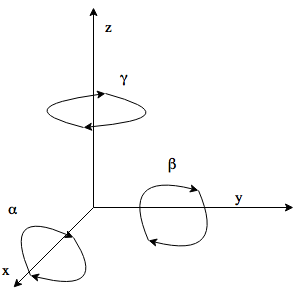
\includegraphics[scale=.7]{coordinateAxes}}
	\caption{Example of coordinate axes and orientation labeling}
\end{figure}

State estimation is all about converting data between the global and local coordinate frames. The global frame is typically the data we want to output, it is the position and orientation of our device with respect to a global origin point, if we were talking about a rocket this could be the launch pad with which the rocket launches from. The local frame is the data with respect to a local origin point which is typically the center of our IMU. 

\begin{figure}[H]
	\centering
	\textbf{Transformation}\par\medskip
	\fbox{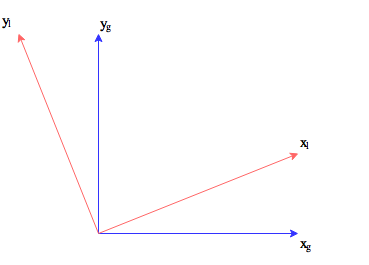
\includegraphics[scale=.7]{LocalToGlobalTransformation}}
	\caption{Transformation between local frame and global frame}
	\label{fig:transform}
\end{figure}
When we receive data from the IMU it is always in reference to the local frame. For example if I have an IMU on my rocket the x axis always points in the direction of the nose cone, no matter which way the rocket rotates in space or accelerates the x axis will always point along the nose cone. In this scenario the rockets x axis points vertically (because the rocket would be pointing up on the launchpad) , while the my x axis (or the global x axis) would be in some horizontal direction parallel to the ground. The question then becomes, how do I tell the rockets position in the global x axis? If I am standing at a launch pad, the rocket launches and moves 2 feet away from me in the global x direction, how am I going to know that if the IMU's local frame is so different from my global frame? The answer is in transformations. Using the rotational data from the gyroscope and the acceleration data from the accelerometer we can create rotational transformation matrices to rotate that data from its local frame to the global frame. 

\begin{center}
\textbf{Rotations}
\end{center}
Lets start with a simple rotation on a 2D axis. We will use x and y. Lets call the x and y magnitudes in the global frame $x_{g}$ and $y_{g}$, while the local frame magnitudes will be $x_{l}$ and $y{l}$. We will start with an example, lets say I have a point which is at (10,8) in the local frame, and I know the local frame has been rotated by 30 degree from the global frame. This example is shown in figure \ref{fig:example1}.

\begin{figure}[H]
	\centering
	\textbf{Transformation Example}\par\medskip
	\fbox{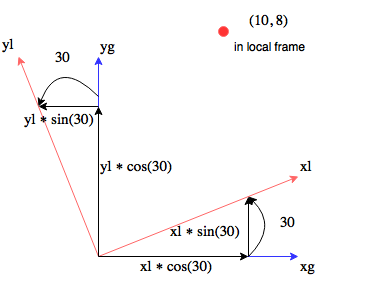
\includegraphics[scale=.7]{TransformationExample}}
	\caption{Example to transform a point from the local frame to the global frame}
	\label{fig:example1}
\end{figure}

Visually you can see that I would have to do some trigonometry to obtain my position in the global frame. First we want to see what my x coordinate would be in the global frame.

Because of the rotation the x component in the local frame exists on both sides of the y axis. So to figure out our global x component we will have to consider the part on the right side of the y axis as well as the left side of the y axis. We can first find the whole component as if it were to the right of the y axis by taking the magnitude of $x_{l}$ multiplied by $cos(\theta)$ which would be $10*cos(30)$. Now we need to subtract out the component to the left of the y axis. If you look carefully you can see that component is equivalent to the magnitude $y_{l}$ multipliled by $sin(\theta)$ which would be $8*sin(30)$.\\\\
We can use the same thought process to calculate the global y component. The global frame will be calculated in 2 parts, first we consider the contribution of the local y axis which is the magnitude of $y_{l}$ multiplied by $cos(\theta)$ or $8*cos(30)$. The second part is the contribution of the local x axis which is the magnitude of $x_{l}$ multiplied by $sin(\theta)$ or $10*sin(30)$. It might be difficult to understand from the explanation above, hopefully you can come to the same conclusion by looking at the figure. Finally you arrive at the equations below:\\

	\begin{align*}
	x_{g} &= 10*cos(30)-8*sin(30) \approx 4.66\\
	y_{g} &= 10*sin(30)+8*cos(30) \approx 11.93
	\end{align*}
From this we infer that the location of the point in the global frame is actually (4.66,11.93)
\begin{figure}[H]
	\centering
	\textbf{Global Frame Coordinate}\par\medskip
	\fbox{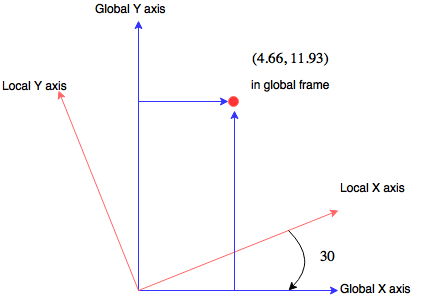
\includegraphics[scale=.7]{GlobalFrameCoordinate}}
	\caption{Final coordinate in the global frame}
	\label{fig:GlobalFrameCoordinate}
\end{figure}

Now that we have completed this example lets try generalizing the equations we came up with. Our rotation angle is $\theta$, local x and y magintudes are $x_{l}$ and $y_{l}$, and our global x and y magnitudes are $x_{g}$ and $y_{g}$.
	\begin{align*}
	x_{g} &= x_{l}cos(\theta)-y_{l}sin(\theta)\\
	y_{g} &= x_{l}sin(\theta)+y_{l}cos(\theta)
	\end{align*}
We can also put this into a matrix form:
\begin{math}
	\begin{bmatrix}
	x_{g}\\
	y_{g}
	\end{bmatrix}=
	\begin{bmatrix}
	cos(\theta)&-sin(\theta)\\
	sin(\theta)&cos(\theta)
	\end{bmatrix}*
	\begin{bmatrix}
	x_{l}\\
	y_{l}
	\end{bmatrix}
\end{math}\\
To generalize even further we can say: $r_{g} = R(\theta)*r_{l}$ where $r_{g}$ is my global position, $r_{l}$ is my local position, and $R(\theta)$ is called a rotation matrix. The conclusion here is that any point in the local frame can be converted to a point in the global frame via a rotational matrix, and all you need to keep track of is how the local frame has rotated ($\theta$) with respect to the global frame. In the next section we will cover 3 dimensional rotations.



%\newpage      Command to start a new page dont forget

\end{document}